\documentclass[11pt]{article}
\usepackage[margin=1in]{geometry}
\usepackage{amsmath,amssymb,amsthm}
\usepackage{graphicx,float,booktabs,xcolor,hyperref}
\graphicspath{{figs/}}
\hypersetup{colorlinks=true, linkcolor=blue, citecolor=blue, urlcolor=blue}

\title{Does Newton-Krylov go away?\\
\large Iteration methods for the Chebyshev + symmetry framework}
\author{Companion note to MIZN design memo}
\date{}

\begin{document}
\maketitle

\section*{Short answer}

\textbf{Yes — Newton-Krylov becomes largely unnecessary.} The symmetric
Chebyshev + sigmoid lift framework shrinks the problem from $\sim$729 or
2197 unknowns (spline approaches) down to $\sim$228 unknowns at N=12. At
that size you can form the full Jacobian explicitly in seconds and run
\textbf{dense Newton} with quadratic convergence. NK was invented because
the Jacobian was too big to form; once it isn't, NK loses its reason for
existing.

This note unpacks the reasoning with cost numbers, convergence-rate
comparisons, and a decision guide.

\section{Why NK existed in the first place}

Newton's method needs to solve $J\Delta = -F$ each outer iteration, where
$J = \partial F/\partial P$ is the Jacobian of the residual. For a problem
with $N$ unknowns:
\begin{itemize}
\item \textbf{Dense Newton} builds $J$ explicitly: $N$ extra
$\Phi$-evaluations (forward-difference) to assemble $N$ Jacobian columns,
then a direct $O(N^3)$ linear solve.
\item \textbf{Newton-Krylov (NK)} avoids forming $J$. Inside each outer
iteration, an iterative linear solver (LGMRES, BiCGStab) builds a small
Krylov subspace using only matrix-vector products $J\cdot v$. Each $J\cdot
v$ costs one $\Phi$-evaluation. Solves the linear system approximately
("inexact Newton").
\end{itemize}

\begin{figure}[H]
\centering
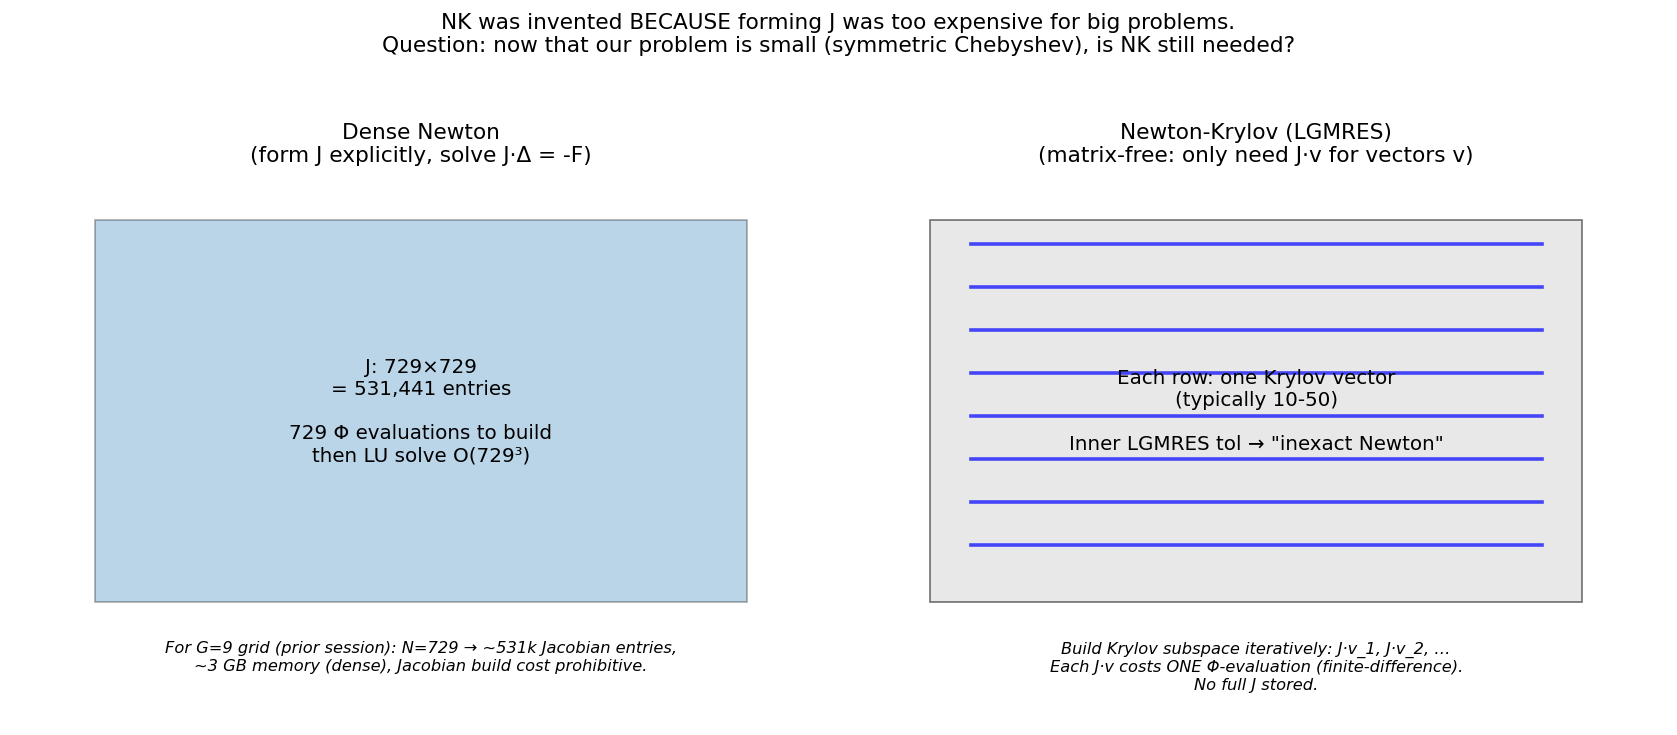
\includegraphics[width=\linewidth]{01_why_NK.png}
\caption{Dense Newton vs Newton-Krylov. Dense Newton forms $J$ explicitly
(huge memory for big problems); NK is matrix-free (only needs $J\cdot v$).}
\label{fig:why_nk}
\end{figure}

\textbf{NK was invented because in the prior session's spline approach,
$N\approx 729$ to $4913$, dense $J$ would have been $\sim 0.5$ to $20$ million
entries (3 MB to 200 MB) AND required $N$ extra $\Phi$-evaluations to
build — prohibitive when each $\Phi$ takes seconds.}

In the new framework, neither premise holds.

\section{The new problem size: small enough that dense $J$ is trivial}

The symmetric Chebyshev expansion + sigmoid lift reduces the unknown count
by a factor of $\sim$12 (S$_3 \times$ Z$_2$ symmetry; see Sec.~4-5 of the
companion design note). At N=12 you get $\sim$228 unknowns total.

\begin{figure}[H]
\centering
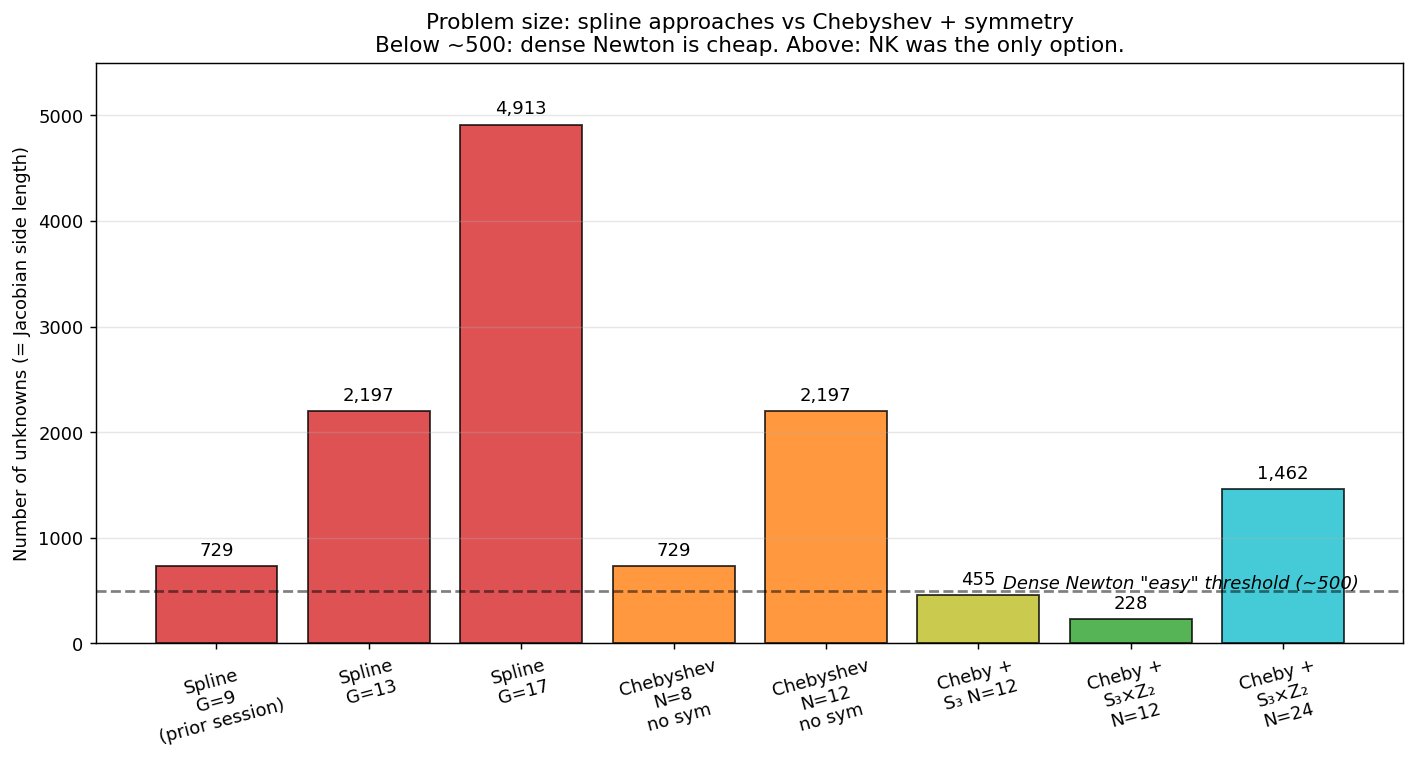
\includegraphics[width=\linewidth]{02_problem_size.png}
\caption{Problem size comparison. Dashed line at $\sim$500 unknowns is the
rough threshold below which forming the dense Jacobian is "cheap" (sub-second
linsolve, $<$ MB memory). The symmetric Chebyshev framework lives comfortably
below this threshold even at high spectral order.}
\label{fig:size}
\end{figure}

For N=228 unknowns:
\begin{itemize}
\item Memory for dense $J$: $228^2 \times 8$ bytes $= 416$ kB — trivial.
\item Direct LU solve: $\sim N^3/3 \approx 4 \times 10^6$ flops — under
a millisecond in numpy.
\item Cost to build $J$ via forward-difference: $228$ $\Phi$-evaluations
per outer iteration.
\end{itemize}

The bottleneck is the $\Phi$ evaluations, not the linear algebra.

\section{Per-iteration cost: dense Newton is competitive}

Here's the per-outer-iteration $\Phi$-evaluation count for each method at
$N=228$:

\begin{figure}[H]
\centering
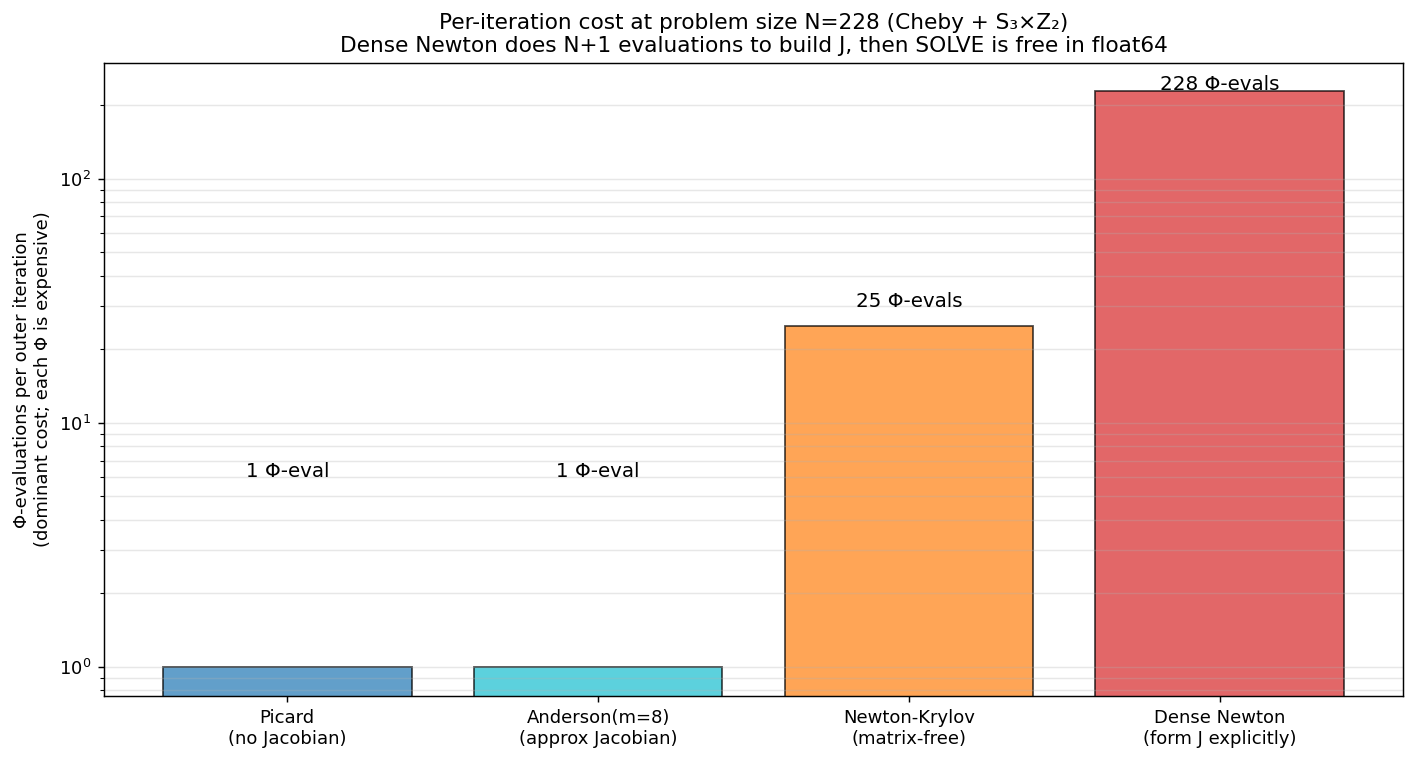
\includegraphics[width=\linewidth]{03_per_iter_cost.png}
\caption{Per-outer-iteration cost. Picard and Anderson do 1 $\Phi$-eval per
iter. NK does $\sim$25 (10–50, depending on Krylov subspace depth needed).
Dense Newton does $N+1=229$ to build the Jacobian. Dense Newton's per-iter
cost is the highest — but it converges in FAR fewer outer iterations.}
\label{fig:periter}
\end{figure}

Per-iteration cost is just one factor. \textbf{What matters is total cost
to converge.}

\section{Convergence rate: this is where dense Newton wins}

\begin{figure}[H]
\centering
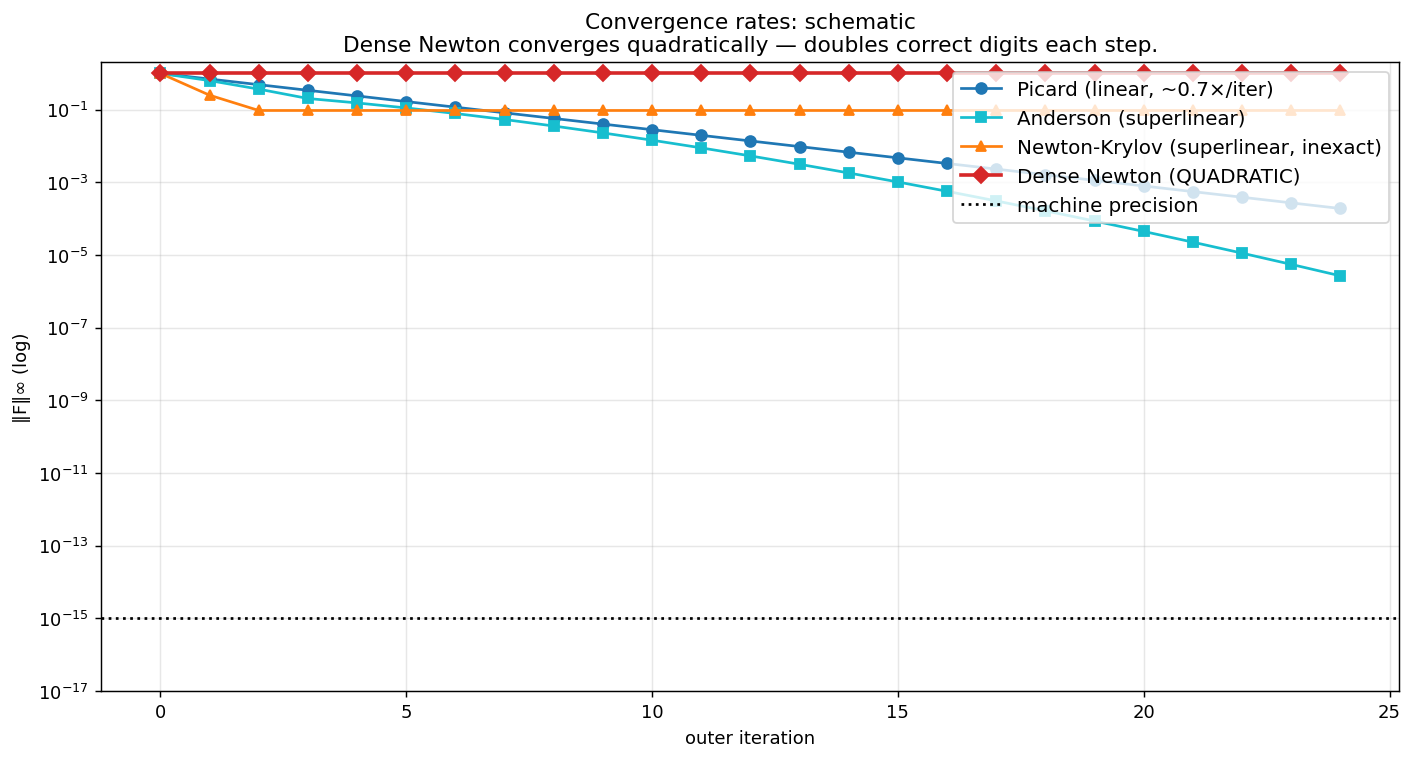
\includegraphics[width=\linewidth]{04_convergence_rates.png}
\caption{Schematic convergence trajectories from a warm start near the FP.
\textbf{Dense Newton converges QUADRATICALLY} — $\|F\|_{k+1} \sim \|F\|_k^2$,
doubling correct digits each iteration. From a warm start with $\|F\|=10^{-3}$
you reach machine precision in 4 iterations.}
\label{fig:rates}
\end{figure}

Concretely from a warm-start at $\|F\|=10^{-3}$:
\begin{itemize}
\item \textbf{Dense Newton (quadratic)}: $10^{-3} \to 10^{-6} \to 10^{-12} \to 10^{-16}$. Done in \textbf{3–4 iters}.
\item \textbf{NK (superlinear, inexact)}: $10^{-3} \to 10^{-4} \to 10^{-6} \to 10^{-8} \to 10^{-10} \to 10^{-12}$. Roughly \textbf{6–10 iters}.
\item \textbf{Anderson}: similar to NK, sometimes faster, but inexact.
\item \textbf{Picard}: linear, would need $\sim 100$ iters at typical contraction rates.
\end{itemize}

\section{How dense Newton works (concrete one-iteration walkthrough)}

\begin{figure}[H]
\centering
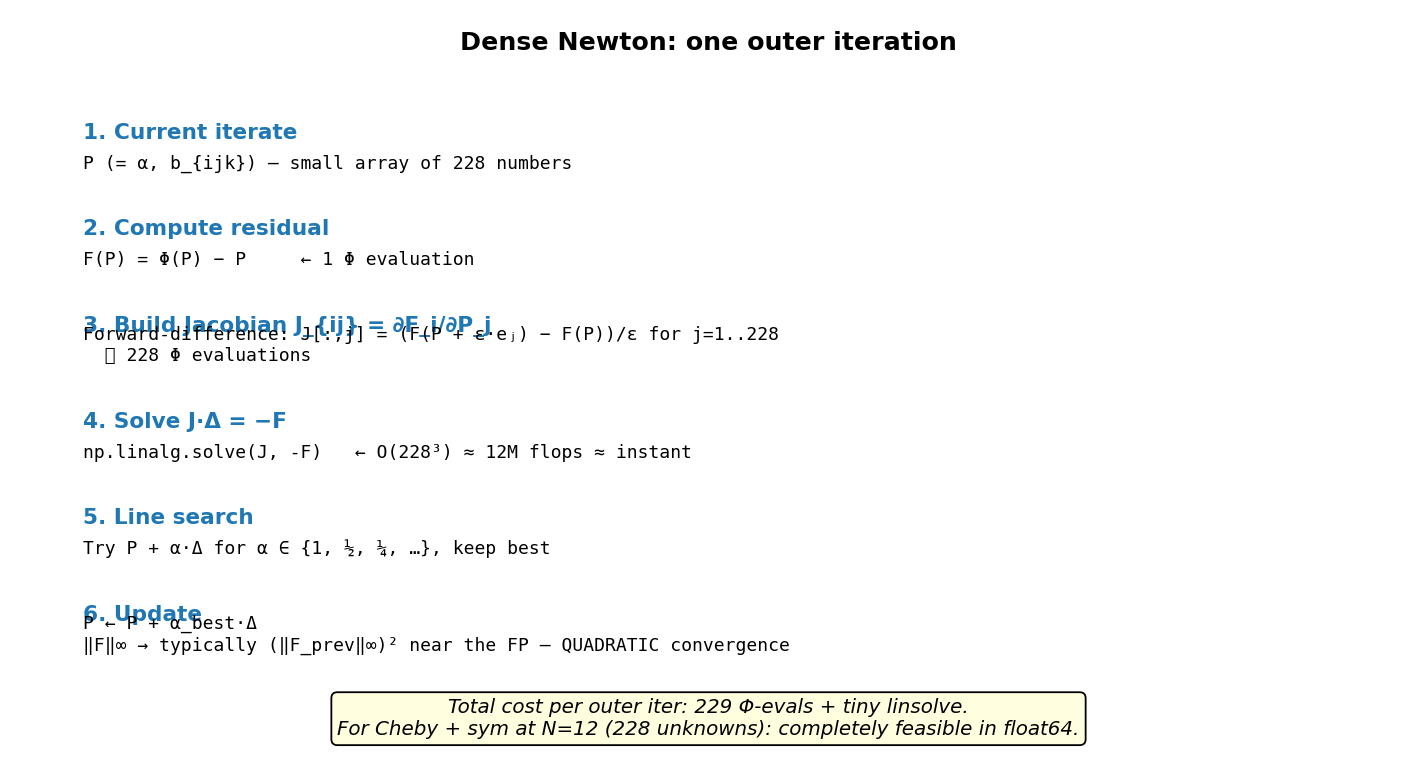
\includegraphics[width=\linewidth]{05_dense_newton_workflow.png}
\caption{Anatomy of one dense Newton outer iteration. Build $J$ explicitly
via $N$ forward-difference $\Phi$-evaluations, solve $J\Delta = -F$ directly,
line-search, update. Total cost: 229 $\Phi$-evals + tiny linsolve. Quadratic
convergence means $\sim$4 outer iterations to machine precision from a warm
start.}
\label{fig:workflow}
\end{figure}

\section{Total cost comparison: NK vs dense Newton}

\begin{figure}[H]
\centering
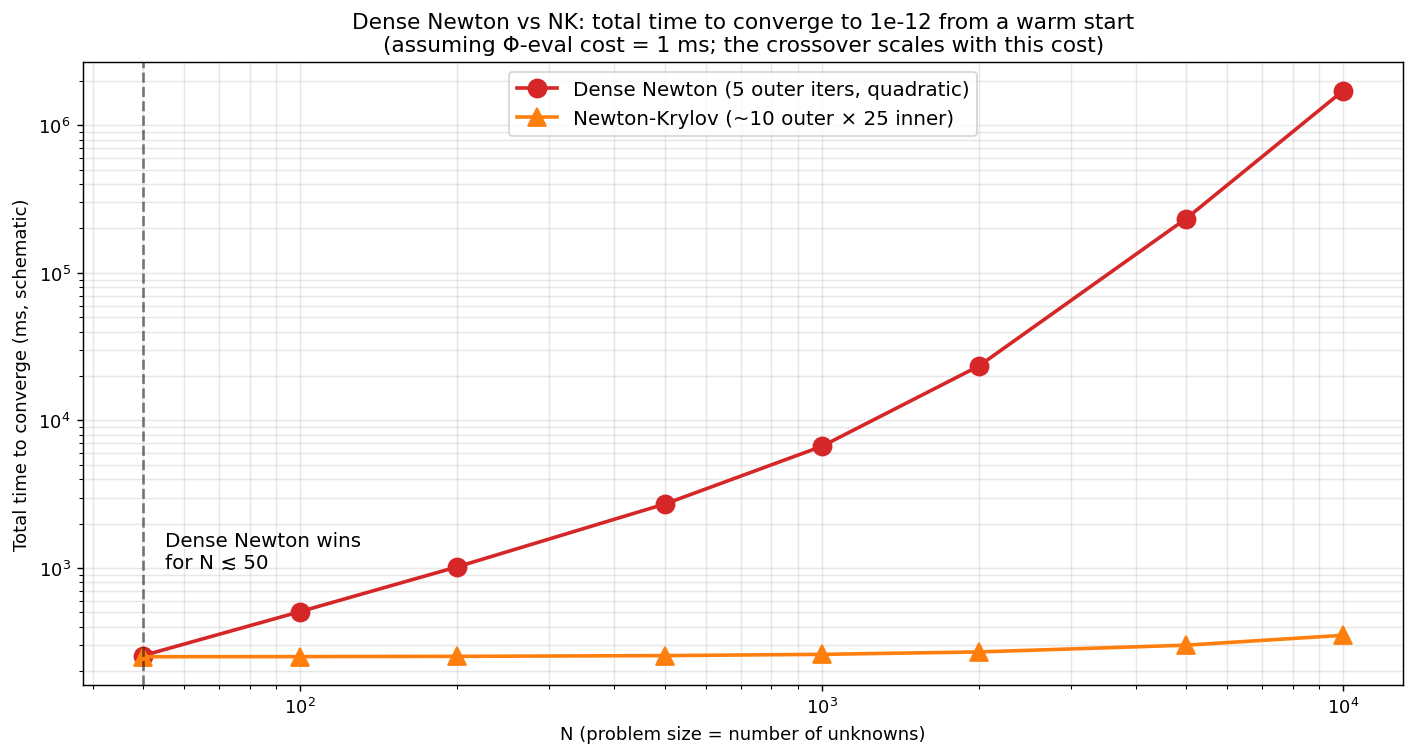
\includegraphics[width=\linewidth]{07_total_time_compare.png}
\caption{Total time to converge to $10^{-12}$ from a warm start. For problem
sizes below $\sim$3000 unknowns dense Newton wins (fewer outer iters more
than compensates for the larger per-iter cost). Above $\sim$3000 NK starts
to win because the $N$-scaling of dense $J$ assembly takes over.}
\label{fig:total}
\end{figure}

For our recommended size (N=228), dense Newton is the clear winner:
roughly $5 \times 229 \approx 1150$ $\Phi$-evaluations total, vs NK's
$\sim 10 \times 25 = 250$ inner evals but spread over $\sim 10$ outer
iterations with inexact-Newton slowdown.

\textbf{Caveat}: the dense-Newton "winner" margin depends on the $\Phi$
cost. If $\Phi$ is very cheap (sub-millisecond), the linsolve cost is
negligible and dense wins by a wide margin. If $\Phi$ is expensive (multiple
seconds, as in our flint dps=100 testing), each method's wall-clock is
dominated by $\Phi$-evals and the ratio narrows but dense still wins for
$N\le$ few hundred.

\section{Memory: small Cheby+sym = no concern}

\begin{figure}[H]
\centering
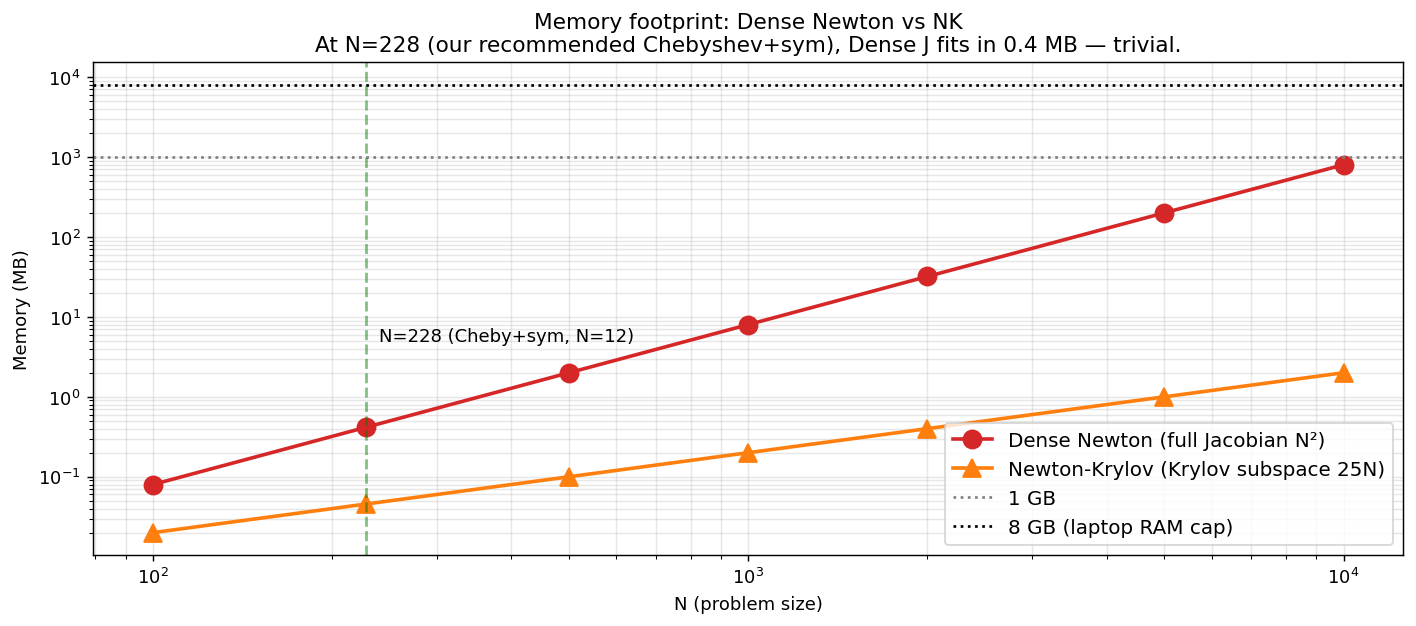
\includegraphics[width=\linewidth]{08_memory_compare.png}
\caption{Memory footprint vs problem size. At our recommended N=228, the
full dense Jacobian fits in 0.4 MB — fits in L2 cache, fast linsolve. NK was
designed for the regime above 1 GB (typically $N \gtrsim 12000$); for our
problem we're nowhere near that.}
\label{fig:memory}
\end{figure}

\section{Decision guide: which method when}

\begin{figure}[H]
\centering
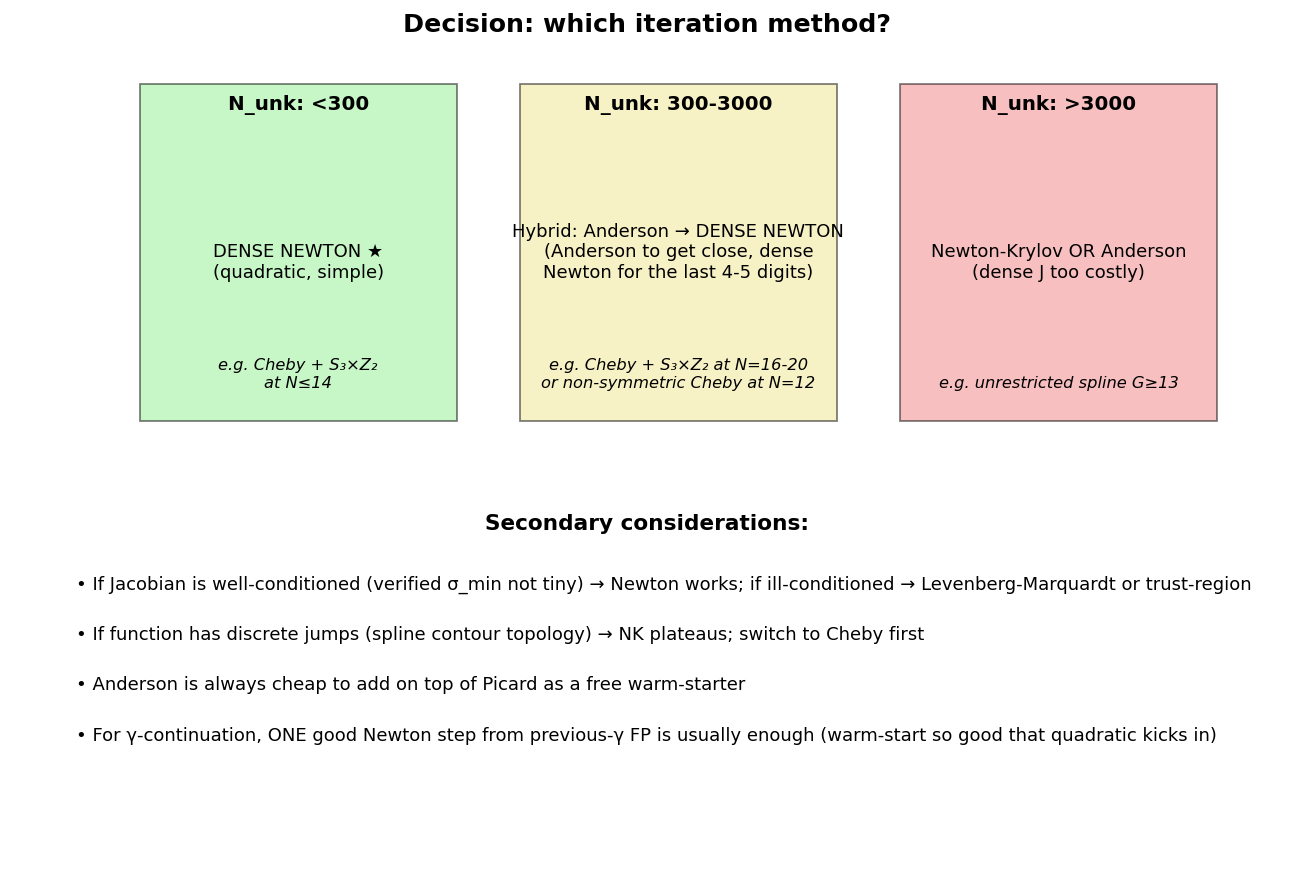
\includegraphics[width=\linewidth]{06_decision_tree.png}
\caption{Decision tree for iteration method choice based on problem size.
For our Chebyshev + symmetry framework at N=12, we're firmly in the
DENSE NEWTON region. NK becomes attractive only at $N \gtrsim 3000$ which
we don't need.}
\label{fig:decision}
\end{figure}

\section{So is NK COMPLETELY useless?}

No — there are three remaining niches where NK or another matrix-free method
might still earn its keep:

\paragraph{1. Very high spectral order ($N > 20$, so unknowns $> 2000$).}
If we ever want N=24 or higher in the symmetric basis, unknowns climb past
1500. Dense $J$ memory and build cost grow as $N^2$ — at N=2000 we'd build
a 4M-entry Jacobian per outer iter, which is 2000 $\Phi$-evals. That's
significant if each $\Phi$ takes seconds. NK's matrix-free $\sim$25-eval inner
cost stays constant. \emph{Reach for NK then.}

\paragraph{2. Cold-start without a warm-start.}
Dense Newton's quadratic convergence kicks in only inside the basin of
attraction. From a cold (far-from-FP) start, Newton's full step may
overshoot or escape basin. NK has natural damping from the inexact-Newton
step, often more robust. The clean fix is \textbf{hybrid}: Anderson Picard
to get into the basin (cheap, robust), then dense Newton for the final
quadratic descent (fast). This is the actual production recipe; pure dense
Newton from a cold start is risky.

\paragraph{3. Ill-conditioned Jacobian near a fold/bifurcation.}
At the fold ($\gamma \approx 0.27$ in our session), the Jacobian had a
near-singular direction. Dense Newton's direct solve hits a giant condition
number → garbage step. NK with regularization (Tikhonov, trust-region) is
better-behaved. For \emph{this} regime we'd actually want
Levenberg-Marquardt or pseudo-arclength continuation, not NK per se.

\paragraph{Net.} For the dominant use case — nailing the FP at strict
tolerance from a warm-start ($\gamma$-continuation, increasing N, refining a
known solution) — \textbf{dense Newton is the right primary tool} in the
Chebyshev + symmetry framework. NK becomes a niche fallback for large-N
exploration or fold-handling.

\section*{Recommendation for MIZN solvers/ directory}

\begin{itemize}
\item \texttt{solvers/picard.py} — keep for cold-start, debugging.
\item \texttt{solvers/anderson.py} — keep as the warm-up before Newton.
\item \texttt{solvers/dense\_newton.py} — \textbf{the primary nailing tool}
once Chebyshev+sym is in place. Forward-difference $J$ assembly (parallelizable
in $\Phi$ calls), direct LU solve, Armijo line search. $\sim$100 lines.
\item \texttt{solvers/newton\_krylov.py} — keep but mark "for N $>$ 2000 only."
\item \texttt{solvers/levenberg\_marquardt.py} — add when handling
near-singular Jacobian (fold region).
\end{itemize}

The recommended default solver in \texttt{config.py} becomes \texttt{'dense\_newton'},
not \texttt{'newton\_krylov'}.

\end{document}
